\chapter{Metodología y rigor}
\section{Método de trabajo}
Se ha utilizado un modelo de desarrollo en cascada \cite{Tfg:waterfall}, ya que es una planificación sencilla, fácil de entender y utilizar por alguien que no está acostumbrado a trabajar siguiendo un método concreto. Para el éxito de este proyecto y utilizando esta metodología, es muy importante la documentación, cosa que es positiva ya que este proyecto luego será utilizado en una empresa y ayudará a que los desarrolladores de la empresa tengan referencias e información sobre diferentes aspectos del proyecto. Al tener desde un principio la mayoría de requisitos del proyecto definidos, era poco probable que surgieran necesidades imprevistas, esto sumado al hecho de que el desarrollo del proyecto lo ha llevado a cabo una única persona y por lo tanto no ha tenido que sincronizarse con otros trabajadores, ha hecho que el modelo cascada sea uno de los más adecuados para este proyecto.

A parte del uso del modelo de desarrollo cascada, la comunicación con el director del trabajo ha sido frecuente, ya sea para hablar de aspectos generales del proyecto, o de aspectos más concretos. La comunicación ha sido vía email o en persona. Se pactaron reuniones con el director cada quince días para comprobar los avances del proyecto. 

\section{Herramientas de seguimiento}
Para el seguimiento del desarrollo del software se ha utilizado el sistema de control de versiones Git y estas versiones se almacenan en un repositorio remoto, se ha utilizado GitHub como repositorio remoto.

Para el seguimiento del diseño e implementación del sistema se ha generado documentación que se publicará en el JIRA de la empresa. Para asegurar que el diseño y la implementación es aparentemente correcta se ha consultará con el director antes de publicar la documentación en JIRA.

Para la generación de documentación de seguimiento se ha utilizado la suite ofimática LibreOffice, también LaTeX y se publicará en JIRA bajo el formato PDF.

\section{Métodos de validación}

Los métodos de validación corresponderían a la fase de validación del desarrollo en cascada.

La parte de implementación del proyecto se puede dividir en las siguientes fases:

\begin{itemize}
	\item Subsistema de recolección y envío de eventos
	\item Subsistema de recepción e ingesta de eventos
	\item Subsistema de transformación de eventos
	\item Integración con JIRA y ES Stack
\end{itemize}

Se ha aplicado el desarrollo en cascada de forma independiente en cada fase del proyecto por lo que se obtienen cuatro fases de validación.

\subsection{Validación del subsistema de recolección y envío}
La fase de validación del subsistema de recolección y envío de eventos consiste en la creación de una sencilla aplicación que integra las librerías escogidas en la fase de diseño con el fin de que recolecte y envíe eventos a un servidor desplegado en un entorno de pruebas. Tal servidor consiste en una máquina virtual que simula ser el subsistema de recepción e ingesta de eventos. Se ha modificado todo aquello de la aplicación que era erróneo hasta que se ha conseguido el resultado esperado en el servidor. Una vez se ha conseguido el resultado esperado, se han exportado las configuraciones a los entornos de producción.

%%Foto de la app del movil con el nombre TFG recolección y envío

En la Figura \ref{fig:android} se puede ver una captura de la aplicación que se ha creado para validar que se recogen y envían los eventos correctamente. Consiste en dos botones, uno que genera un crash y otro que genera un log con el texto que se le ponga en la textbox. Luego la aplicación, en el caso del crash lo envía al módulo de recepción sin almacenarlo en el dispositivo, y en el caso del log lo almacena en el dispositivo hasta que lo envía cuando la aplicación se cierra.

\begin{figure}[!htb]
	\centering
	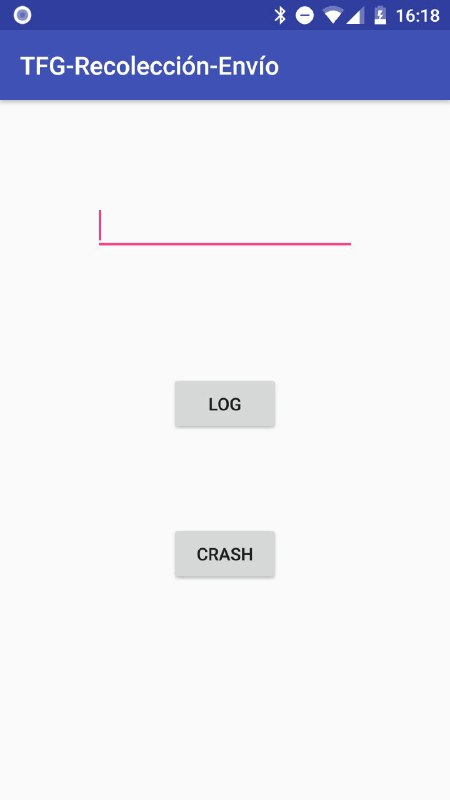
\includegraphics[scale=0.40] {captura.jpeg}
	\caption{Captura de la aplicación de validación}
	\label{fig:android}
\end{figure}

\subsection{Validación del subistema de recepción e ingesta}
La fase de validación del subistema de recepción e ingesta de eventos consiste en, por un lado configurar en una máquina virtual el módulo de recepción para que sea capaz de recibir eventos y pasarlos al módulo de ingesta. Por otro lado se ha de configurar en otra máquina virtual el módulo de ingesta de eventos para que sea capaz de comunicarse con el módulo de recepción de eventos y almacenar de forma parcial los eventos. Una vez las dos máquinas virtuales se comuniquen entre si, y los mensajes enviados al módulo de recepción se almacenen en el módulo de ingesta, se ha considerado que la configuración principal era la correcta y se ha procedido a exportar tal configuración al entorno de producción.

%%Foto con output de la petición POST y foto con output del topic logs y crashes


En la Figura \ref{fig:POST} se puede ver la respuesta positiva que da el módulo de recepción a la petición HTTP POST para publicar datos en el módulo de ingesta. El código 200 de HTTP indica que el comportamiento es esperado. A parte del código 200, se ofrece información sobre como se han distribuido los datos en el módulo de ingesta, cosa que ayuda a validar el módulo de ingesta, en la Figura \ref{fig:POST} se puede ver tal información.

\begin{figure}[!htb]
	\centering
	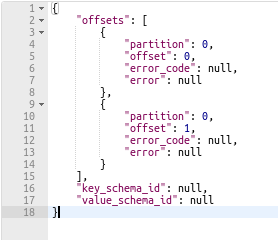
\includegraphics[scale=0.60] {kafka-rest.png}
	\caption{Cuerpo de la respuesta HTTP del módulo de recepción}
	\label{fig:POST}
\end{figure}


En la Figura \ref{fig:logs} se ve el contenido del topic logs y en la Figura \ref{fig:crashes} el contenido del topic crashes. Si los logs y los crashes que se generan con la aplicación aparecen en sus respectivos topics es que tanto el módulo de recepción como el de ingesta están funcionando correctamente.

\begin{figure}[!htb]
	\centering
	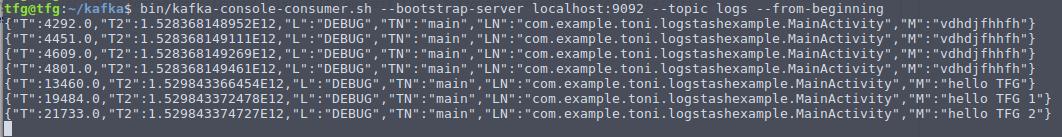
\includegraphics[scale=0.60, width=\linewidth] {kafka-logs.png}
	\caption{Contenido del topic logs}
	\label{fig:logs}
\end{figure}


\begin{figure}[!htb]
	\centering
	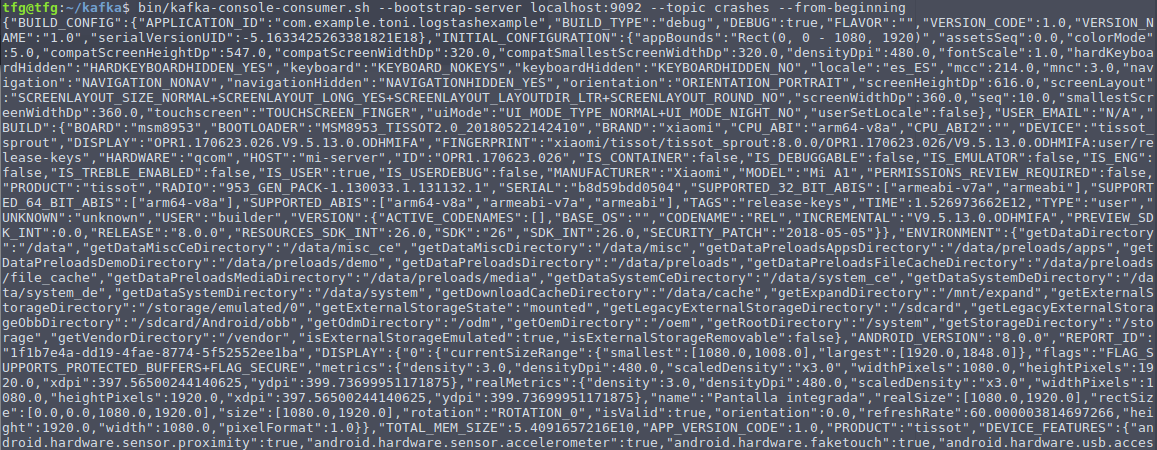
\includegraphics[scale=0.60, width=\linewidth] {kafka-crashes.png}
	\caption{Contenido del topic crashes}
	\label{fig:crashes}
\end{figure}

\subsection{Validación del subsistema de transformación}
La fase de validación del subsistema de transformación de eventos, consiste en lanzar las aplicaciones de procesado y configurar en local una máquina virtual con el subsistema de recepción e ingesta de eventos a la cual se han ido enviando eventos, tales eventos van a ser consumidos por la aplicación de procesado que se ha programado y por Logstash, se ha redirigido la salida de tales aplicaciones a la consola para validar que la transformación es la correcta, una vez se han obtenido los datos esperados, se ha procedido a desplegar las configuraciones en entornos de producción.

%%Foto output kafka streams logstash

En la Figura \ref{fig:crashout} se puede ver el resultado de la transformación de Kafka Streams, el formato del mensaje es el esperado, por lo que se puede dar por validado.

\begin{figure}[!htb]
	\centering
	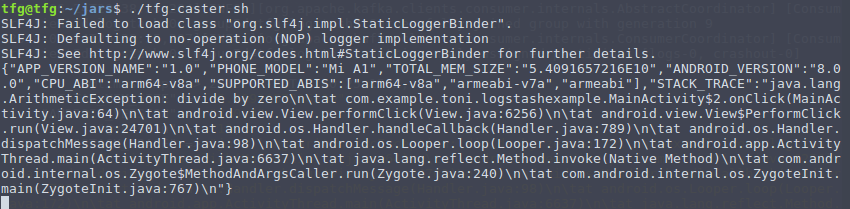
\includegraphics[scale=0.60, width=\linewidth] {crashout.png}
	\caption{Resultado de la transformación con Kafka Streams}
	\label{fig:crashout}
\end{figure}

En la Figura \ref{fig:logstash} se ve como queda el mensaje una vez ha sido transformado por Logstash, como el formato del mensaje es el esperado, se puede dar por validado.

\begin{figure}[!htb]
	\centering
	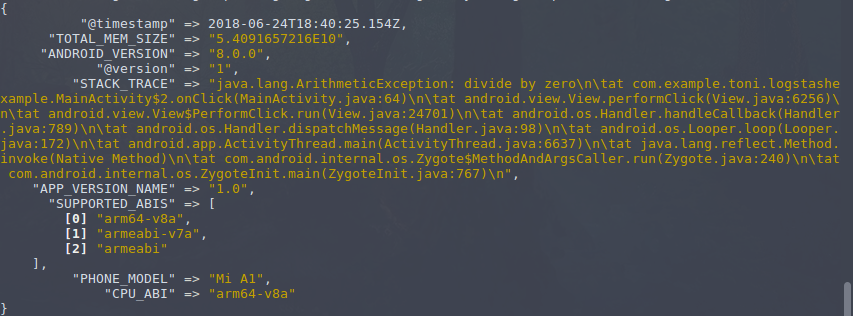
\includegraphics[scale=0.60, width=\linewidth] {logstash.png}
	\caption{Resultado de la transformación con Logstash}
	\label{fig:logstash}
\end{figure}




\subsection{Validación de la integración con JIRA y ELK Stack}
La fase de validación de la integración con JIRA y ELK Stack consiste en montar en local los tres subsistemas, un nodo con JIRA y un nodo con toda la ELK Stack, refinar las configuraciones de los módulos hasta que se consiga, recolectar, enviar, recibir, ingerir, transformar y cargar un evento en JIRA y en la ELK Stack. En JIRA se tendrá que generar un ticket con información sobre el evento. En ls ELK Stack, Logstash ya ha hecho una transformación del evento, lo pasará a Elastic Search, y Kibana será capaz de consumir el evento apuntando a Elastic Search. Una vez se ha conseguido el comportamiento deseado, se han exportado las configuraciones a los entornos de producción.

En la Figura \ref{fig:jira} se puede ver el ticket en JIRA que se ha creado fruto de los crashes que se han generado.

\begin{figure}[H]
	\centering
	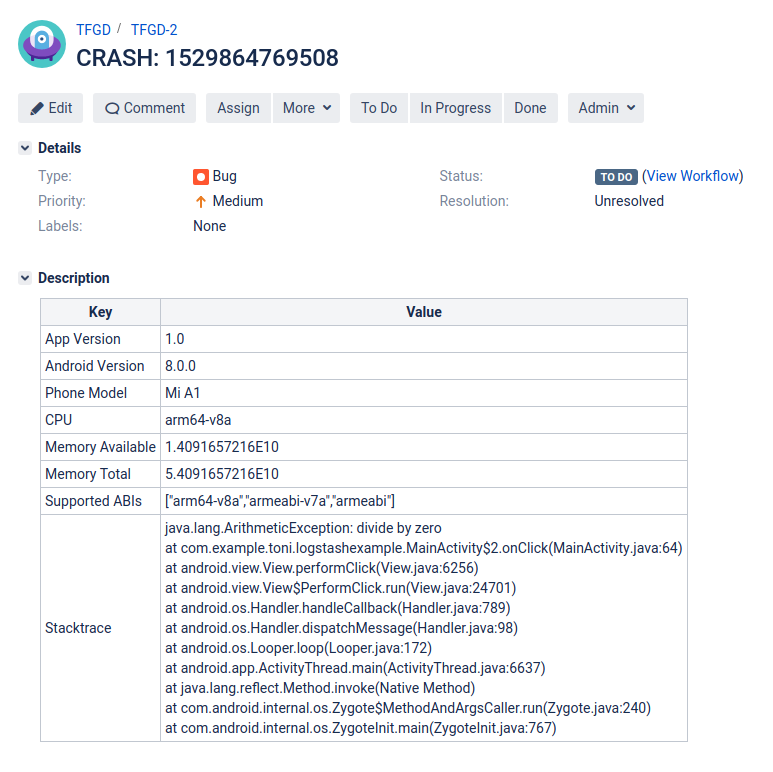
\includegraphics[scale=0.4] {jira.png}
	\caption{Ticket resultante en JIRA}
	\label{fig:jira}
\end{figure}

En la Figura \ref{fig:kibana} se ve diferentes resultados en Kibana que se han creado fruto de los eventos que se han generado.

\begin{figure}[H]
	\centering
	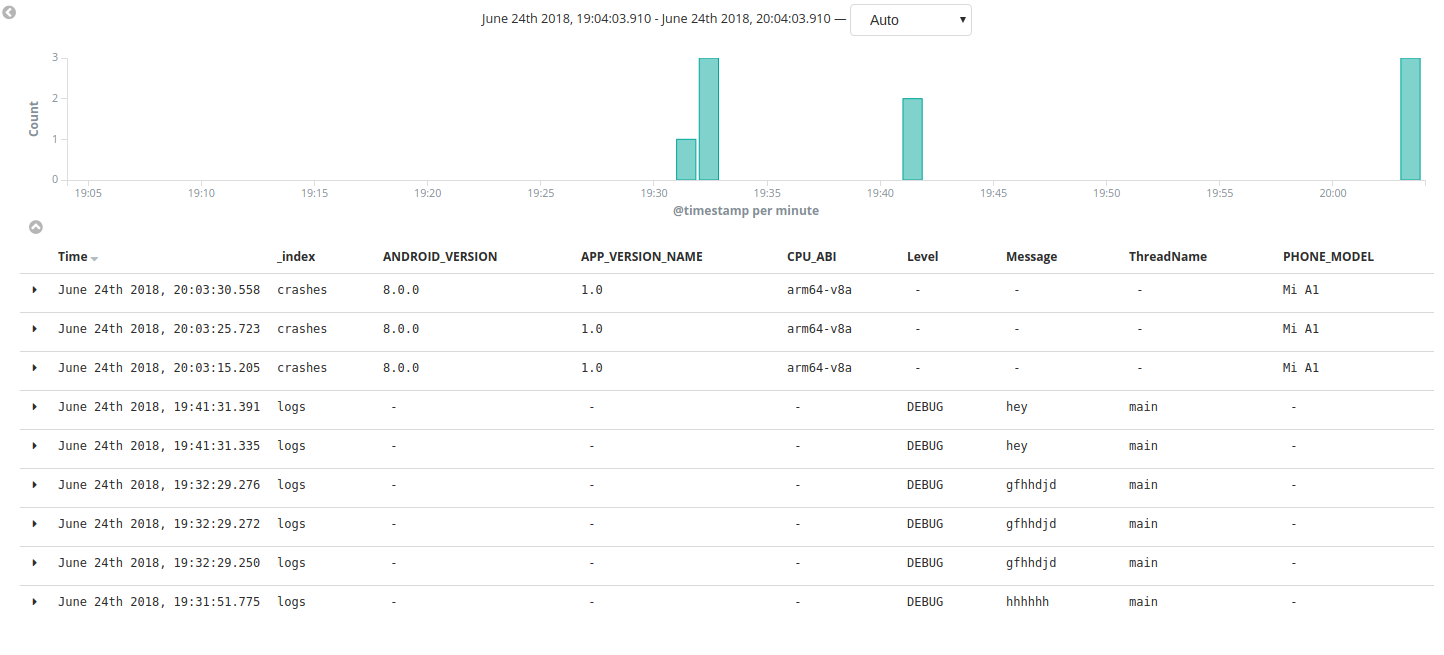
\includegraphics[scale=0.5, width=\linewidth] {kibana.png}
	\caption{Resultados generados por los eventos}
	\label{fig:kibana}
\end{figure}

Puesto que el ticket en JIRA existe, y los resultados en Kibana también, significa que todos los módulos del sistema funcionan correctamente y se puede dar por validado la totalidad el sistema.

Una vez han estado todos los módulos corriendo en producción, también se ha testeado que se cumpla el comportamiento esperado. Para ello se han generado una serie de eventos, los cuales han de seguir el pipeline hasta llegar a JIRA y Kibana. Cuando JIRA y Kibana han mostrado lo deseado se ha concluido el testeo.

Además de tales pruebas y para asegurar el correcto avance del diseño del proyecto, se ha mantenido un contacto frecuente con el director para que vaya dando su visto bueno. Todas las pruebas y tests las ha llevado a cabo el desarrollador del proyecto.